\title{Midterm 3}
\author{Dr. Jordan Hanson - Whittier College Dept. of Physics and Astronomy}
\date{\today}
\documentclass[10pt]{article}
\usepackage[a4paper, total={18cm, 27cm}]{geometry}
\usepackage{outlines}
\usepackage{graphicx}
\begin{document}
\maketitle

\section{Memory Bank}

\begin{enumerate}
\item $\vec{E} = -\frac{\Delta V}{\Delta x}$ ... E-field is the slope or change in voltage with respect to distance
\item $V(x) = -E x + V_0$ ... Voltage is linear between two charge planes
\item $Q = CV$ ... Definition of capacitance
\item $C = \frac{\epsilon_0 A}{d}$ ... Capacitance of a parallel plate capacitor
\item $C_{tot}^{-1} = C_1^{-1} + C_2^{-1}$ ... Adding two capacitors \textit{in series.}
\item $C_{tot} = C_1 + C_2$ ... Adding two capacitors \textit{in parallel.}
\item $i(t) = dQ/dt$ ... Definition of current.
\item $v_d = i/(nqA)$ ... Charge drift velocity in a current $i$ in a conductor with number density $n$ and area $A$.
\item $R_{tot}^{-1} = R_1^{-1} + R_2^{-1}$ ... Adding two capacitors \textit{in parallel.}
\item $R_{tot} = R_1 + R_2$ ... Adding two capacitors \textit{in series.}
\item $\Delta V = I R_{\rm tot}$, $\vec{J} = \sigma \vec{E}$ ... Versions of Ohm's Law. ($\vec{J}$ is the current density with units of Amps per meter-squared).
\item $P = I V$ ... Relationship between power, current, and voltage.
\item $V_{\rm C}(t) = \epsilon_1 \left(1 - \exp(-t/\tau)\right)$ ... voltage across the capacitor in an RC series circuit.  The time constant $\tau = RC$.
\item $i(t) = \frac{\epsilon_1}{R} \exp(-t/\tau)$ ... Current in an RC series circuit.
\item $i_{\rm in} = i_{\rm out}$ ... Kirchhoff's junction rule.
\item $\epsilon_1 + \epsilon_2 + \epsilon_3 + ... = 0$ ... Kirchhoff's loop rule.
\item $\vec{F} = q\vec{v} \times \vec{B}$ ... The Lorentz force on a charge $q$ with velocity $\vec{v}$ in a magnetic field $\vec{B}$.
\item $\vec{F} = I\vec{L} \times \vec{B}$ ... The Lorentz force on a conductor of length $\vec{L}$ carrying a current $I$ in a magnetic field $\vec{B}$.
\item $\int \vec{B} \cdot d\vec{l} = \mu_0 I_{enc}$ ... Amp\`{e}re's Law.
\item $\epsilon = -N d\phi/dt$ ... Faraday's Law.
\item $\phi = \vec{B} \cdot \vec{A}$ ... Definition of magnetic flux.
\item $-N d\phi/dt = \oint \vec{E} \cdot d\vec{l}$ ... Induced E-field due to changing magnetic flux.
\item Faraday's Law using \textbf{Inductance}, M: $emf = -M \frac{dI}{dt}$.
\item Typically, we refer to \textit{mutual inductance} between two objects as $M$, and \textit{self inductance} as $L$.  Self-inductance: $\Delta V = -L (dI/dt)$.
\item Units of inductance: V s A$^{-1}$, which is called a Henry, or H.
\item $B = \mu_0 n I$ ... The B-field of a solenoid, $n = N/L$ is the turn density, and $I$ is the current.
\end{enumerate}

\clearpage

\section{Chapter 11: Magnetic Forces and Fields}

\begin{figure}
\centering
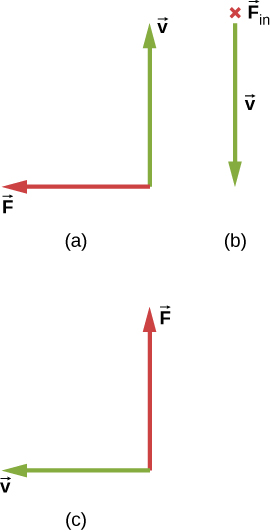
\includegraphics[width=0.2\textwidth]{bfield1.jpeg} \hspace{0.5cm}
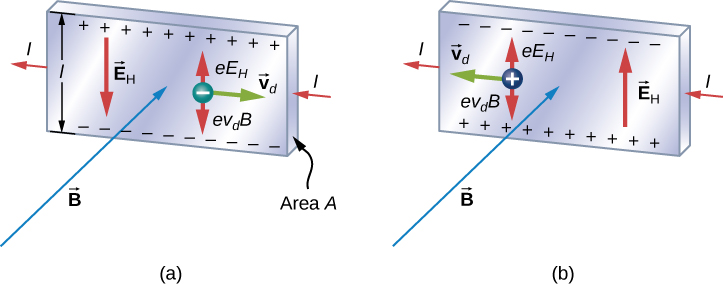
\includegraphics[width=0.5\textwidth]{hallEffect1.jpeg}
\caption{\label{fig:chap11_1} (Left) A current $I$ experiences a force $F$ in a B-field.}
\end{figure}

\begin{enumerate}
\item Consider Fig. \ref{fig:chap11_1} (left).  In each of the three cases, determine the direction of the B-field given that F is the Lorentz force.
\begin{itemize}
\item a:
\item b:
\item c:
\end{itemize}
\item Consider Fig. \ref{fig:chap11_1} (right).  \textbf{The Hall Effect}.  An E-field exists in the vertical direction and a B-field is perpendicular to the direction of charge velocity.  (a) Show that if the E-field force on a charge balances the Lorentz force on a charge, that $v = E/B$. (b) If the E-field is constant, $E = \Delta V/\Delta x$.  Show that
\begin{equation}
\Delta V = \frac{B\Delta x I}{n q_e A}
\end{equation}
where $n$ is the charge carrier density, $q_e$ is the electron charge, $A$ is the cross-sectional area of the conductor, and $I$ is the current.  Plug in $B = 1.33$ T, $\Delta x = 2$ cm, $I = 10$ A, $n = 2 \times 10^{28}$ m$^{-3}$, $A = 1$ mm$^2$, and $q_e$ is the charge of an electron. \\ \vspace{2.5cm}
\item A proton has a magnetic field due to its spin. The field is similar to that created by a circular current loop $0.65 \times 10^{-15}$ m in radius with a current of $1.05 \times 10^{4}$ A.  Find the maximum torque on a proton in a 2.50-T field. (This is a significant torque on a small particle.) \\ \vspace{1cm}
\end{enumerate}

\section{Chapter 12: Sources of Magnetic Fields}

\begin{figure}[ht]
\centering
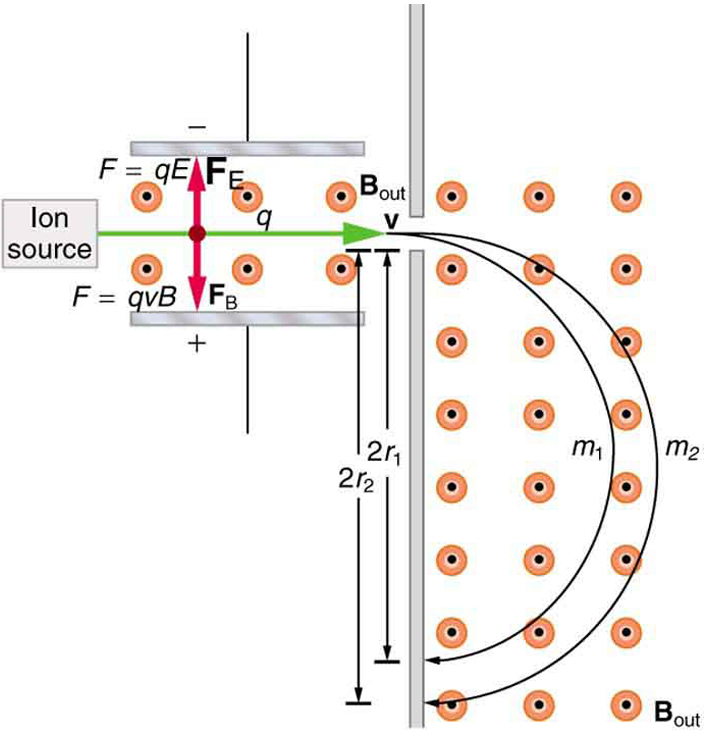
\includegraphics[width=0.35\textwidth]{vsel.jpeg}
\caption{\label{fig:chap12_1} A basic diagram of a \textit{toroid}, which is a solenoid wrapped into a circular tube.}
\end{figure}

\begin{enumerate}
\item (a) What is the B-field inside a solenoid with 500 turns per meter, carrying a current of 0.3 A? (b) Suppose we insert a piece of metal inside the solenoid, boosting $\mu_0$ by a factor of 5000.  What is the new B-field?  \\ \vspace{3cm}
\item Consider Fig. \ref{fig:chap12_1}.  \textbf{Mass spectrometer}.  Suppose that the 	velocity of the charged particles moving to the right is $v = E/B$.  (a) Show that if $v = E/B$, $F_{net} = 0$ in the region in the top left\footnote{Molecules that do not have this velocity will hit the sides of this portion of the instrument.}.  (b) Recall that the centripetal force on a particle of mass $m$ is $mv^2/r$.  Set this equal to the magnitude of the Lorentz force to prove that 
\begin{equation}
r = \frac{m E}{q B^2}
\end{equation}
The mass of an oxygen nucleus is 16 times that of a proton (mass of proton: $1.67 \times 10^{-27}$ kg).  Suppose oxygen ions with the charge of 1 proton are sent through the mass-sepctrometer.  The E-field is $10$ V/m, and the B-field is $0.01$ T.  What is the distance $r$?
\\ \vspace{1cm}
\end{enumerate}

\section{Chapter 13: Electromagnetic Induction}

\begin{figure}[hb]
\centering
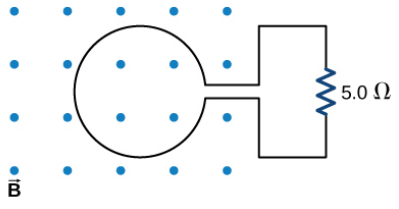
\includegraphics[width=0.25\textwidth]{loopsine.png}
\caption{\label{fig:chap13_1} A voltage is induced on a loop by a changing B-field.}
\end{figure}

\begin{enumerate}
\item The magnetic field in Fig. \ref{fig:chap13_1} flows out of the page through a single ($N=1$) loop, and is tuned to follow the form
\begin{equation}
B(t) = B_0\left( \frac{1}{2} + \frac{2}{\pi}\sin(2\pi f t) + \frac{2}{3\pi}\sin(6\pi f t) + \frac{2}{5\pi}\sin(10\pi f t) \right)
\end{equation}
The loop has a radius $r$.  (a) In terms of the given variables, what is the induced voltage in the circuit? (b) If $B_0 = 0.1$ T, $r = 0.1$ m, and $f = 10^3$ Hz, what is the induced emf at $t=0$?  (c) What is the current through the resistor at $t=1$ ms? \\ \vspace{3cm}
\end{enumerate}

\section{Chapter 14: Inductance}

\begin{enumerate}
\item What is (a) the rate at which the current though a 0.50-H coil is changing if an emf of 0.150 V is induced across the coil? \\ \vspace{1cm}
\item When a camera uses a flash, a fully charged capacitor discharges through an inductor. In what time must the 0.100-A current through a 2.00-mH inductor be switched on or off to induce a 500-V emf?
\end{enumerate}

\end{document}